
\chapter{Referencial Teórico}

\section{Arquitetura de Processadores}

CPU

\section{Controladores de Dispositivos Externos}

CPU

\section{Sistemas Operacionais}

CPU

\section{Carregadores}

CPU

\section{Ligadores}

%Após arquivos objeto de um ou vários módulos de compilação serem gerados por um montador, é preciso combiná-los em um único arquivo que pode ser carregado para a memória por um programa carregador do sistema operacional.



\section{Montadores}

Montadores são programas que traduzem um módulo de compilação em linguagem \textit{assembly} para uma versão em linguagem de máquina. O armazenamento desta versão é feito em um arquivo objeto. Como veremos em uma seção adiante, um arquivo objeto é uma versão binária de um módulo de compilação, que geralmente fica a um passo de poder ser carregada para execução.

\subsection{Linguagem de máquina}

Anteriormente vimos que uma linguagem de montagem, ou linguagem \textit{assembly}, é formada por símbolos mnemônicos, ou palavras-chave, que identificam as instruções que um processador é capaz de executar.

A etapa seguinte à compilação é a montagem. Nesta etapa, é necessário traduzir os mnemônicos \textit{assembly} para sequências de \textit{bits}. Um \textit{bit} é um dígito que pode assumir apenas o valor 0 (zero) ou o valor 1 (um). Durante a execução de um programa, estas sequências de \textit{bits} serão diretamente interpretadas por uma \textit{CPU}.

Costuma-se dizer que a etapa de montagem é onde está localizada a interface \textit{software}-\textit{hardware}. Uma \textit{ISA} - \textit{Instruction Set Architecture}, ou Arquitetura de Conjunto de Instruções - é uma especificação das instruções que uma implementação de processador digital deve fornecer. Esta especificação, entre outras coisas, estabelece os formatos que as sequências de \textit{bits} geradas por montadores devem seguir. Este é o principal conhecimento necessário para construir um montador.

\begin{figure}[ptb]
  \begin{center}
    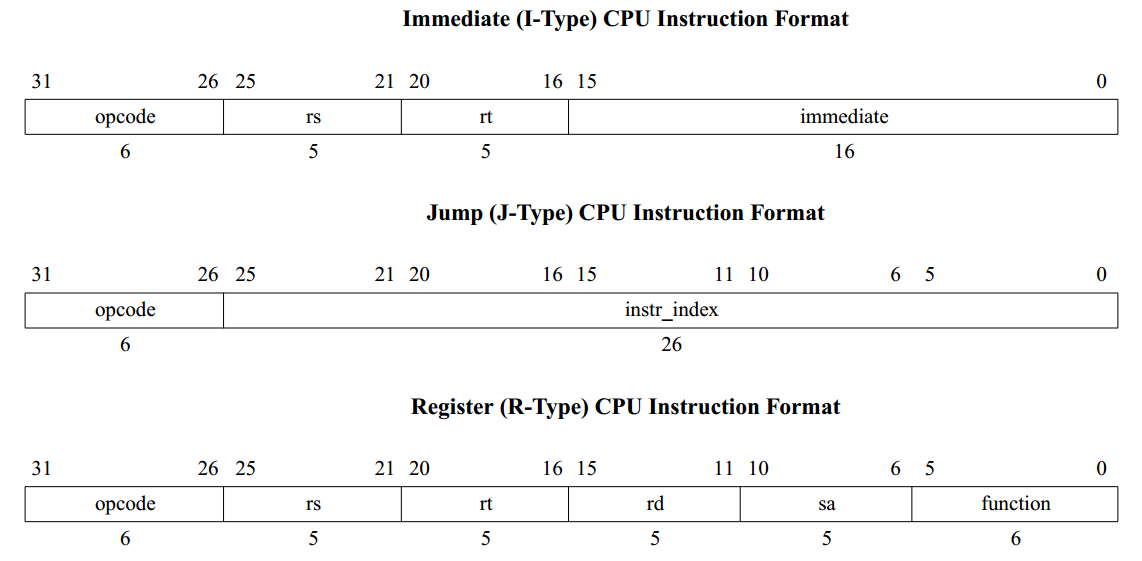
\includegraphics[scale=.45]{imagens/instrucoes_mips}
  \end{center}
  \caption{Os três formatos principais da \textit{ISA} \textit{MIPS32}.}
  \label{instrucoes_mips}
\end{figure}

A figura \ref{instrucoes_mips} mostra os três formatos principais de instruções da arquitetura \textit{RISC} \textit{MIPS32}. Grandes quantidades de instruções se encaixam em cada um dos três formatos. Nesta arquitetura, toda e qualquer instrução ocupa uma palavra de 32 \textit{bits}.

A figura \ref{instrucoes_ia32} mostra o formato geral para uma instrução qualquer da arquitetura \textit{CISC} \textit{IA-32}, criada pela Intel. Nesta arquitetura, o tamanho das instruções vai de 1 até 17 \textit{bytes} (um \textit{byte} são exatamente 8 \textit{bits}).

Com o conhecimento de como cada mnemônico deve ser convertido para código de máquina, podemos construir um montador para uma determinada arquitetura de processadores. À seguir, descrevemos os algoritmos clássicos de montagem.

\begin{figure}[ptb]
  \begin{center}
    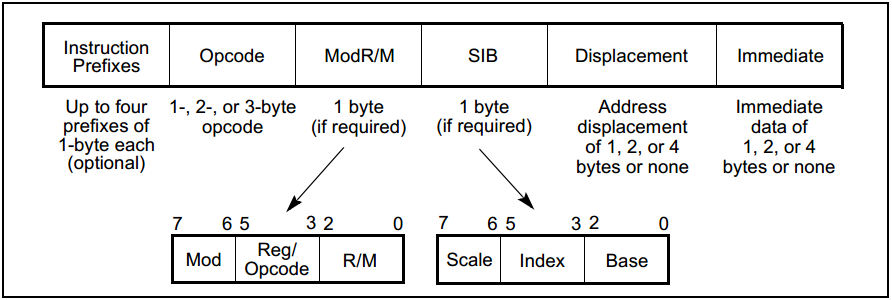
\includegraphics[scale=.6]{imagens/instrucoes_ia32}
  \end{center}
  \caption{Formato geral de uma instrução da \textit{ISA} \textit{IA-32}.}
  \label{instrucoes_ia32}
\end{figure}

\subsection{Algoritmos de montagem}



\section{Compiladores}

CPU

\section{Criptografia}

CPU
